\chapter{Anhang} \label{app:anhang}

\section{Auszug aus dem Datenblatt SN65HVD230} \label{app:anhang_1}
\begin{figure}[!ht]
	\centering
	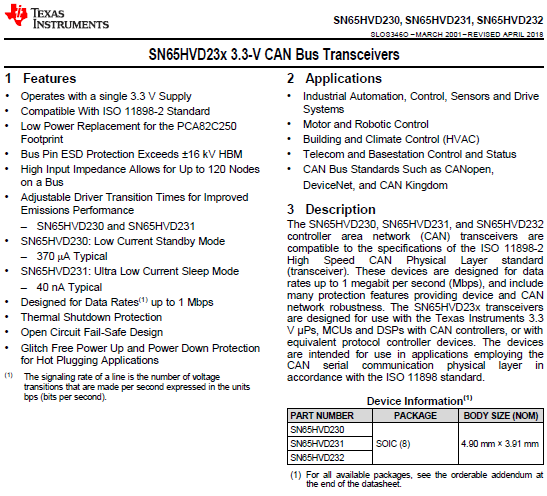
\includegraphics[width=\textwidth]{./SN65HVD230_Datasheet_Seite1}
	\label{abb:SN65HVD230_Datasheet1}
\end{figure}

\begin{figure}[!hp]
	\centering
	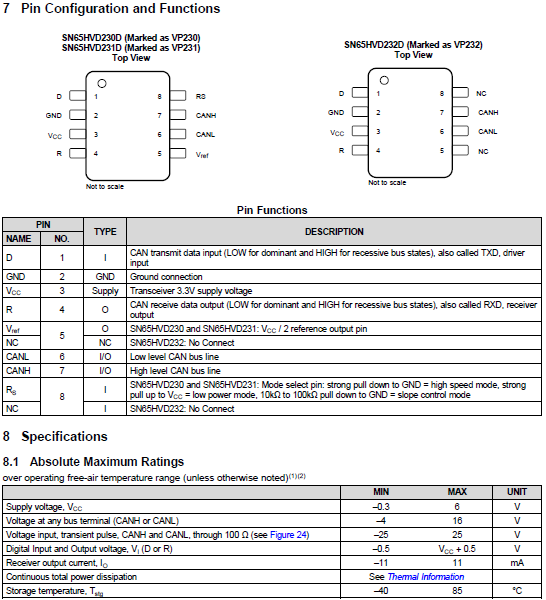
\includegraphics[width=\textwidth]{./SN65HVD230_Datasheet_Seite2}
	\label{abb:SN65HVD230_Datasheet2}
\end{figure}
\newpage

% Hier beginnt neue section: ANhang A2, wird aber im Befehl includepdf gesetzt, sonst wird neue Seite angelegt

\includepdf[pages=1,pagecommand=\section{Einarbeitungsleitfaden Projekt EVObot}]{004_schluss/Einarbeitungsleitfaden}

\includepdf[pages=2-,pagecommand={}]{004_schluss/Einarbeitungsleitfaden}
